\documentclass[xcolor=dvipsnames,9pt]{beamer}
%\usetheme[hideallsubsections]{Hannover}
\usetheme{Hannover} % plenty of themes to pick from
\graphicspath{{../../images/}}
\usepackage[utf8]{inputenc}
\usepackage[T1]{fontenc}
\usepackage{amsmath}
\usepackage{amsfonts}
\usepackage{amssymb}
\usepackage{graphicx}
\usepackage{textpos}
\usepackage{multicol}
\usepackage{tikz}
\usepackage{verbatim}
\usetikzlibrary{arrows,shapes}
\usecolortheme{crane} % plenty of color themes to pick from
\useinnertheme{rectangles}

\definecolor{UBCgreen}{RGB}{30, 77, 43} % UBC Blue (primary)
\definecolor{UBCgold}{RGB}{200, 195, 114} % UBC Grey (secondary)

\setbeamercolor{palette primary}{bg=UBCgreen,fg=white}
\setbeamercolor{palette secondary}{bg=UBCgreen,fg=white}
\setbeamercolor{palette tertiary}{bg=UBCgreen,fg=white}
\setbeamercolor{palette quaternary}{bg=UBCgreen,fg=white}
\setbeamercolor{structure}{fg=UBCgreen} % itemize, enumerate, etc
\setbeamercolor{section in toc}{fg=UBCgreen} % TOC sections
\setbeamercolor{subsection in head/foot}{bg=UBCgold,fg=white}
\setbeamercolor{section in sidebar}{fg=UBCgreen}
\setbeamercolor{section in sidebar}{fg=UBCgreen}
\setbeamertemplate{footline}{}
\setbeamertemplate{page number in head/foot}[totalframenumber]
\setbeamertemplate{navigation symbols}{\footnotesize\usebeamertemplate{page number in head/foot}}
\setbeamertemplate{frametitle}[default][left,colsep=-4bp,rounded=false]
\addtobeamertemplate{frametitle}{}{%
    \begin{textblock*}{100mm}(0.95\textwidth,-0.95cm)
    
\includegraphics[width=0.925cm]{CSU-Ram-357-617.pdf}
    \end{textblock*}
}
\setbeamertemplate{section in toc}{\hspace*{0em}\inserttocsection}
\setbeamertemplate{subsection in toc}{\hspace*{2em}\inserttocsubsection}

\newcommand{\TT}{Transition from 2D to 1D topological superconductivity in a triangular p-wave superconductor island}
\newcommand{\MO}{Motivation}
\newcommand{\DE}{Derivation}
\newcommand{\RE}{Results}
\newcommand{\CO}{Conclusion}

\title{\TT}
\subtitle{}
\author{Aidan Winblad}
\institute{Colorado State University}
\date{\today}

\begin{document}

  \begin{frame}
    \begin{textblock*}{100mm}(0.45\textwidth,-0.75em)
      
\includegraphics[width=1cm]{CSU-Ram-357-617.pdf}
    \end{textblock*}
  \titlepage
  \end{frame}

  \begin{frame}
  \frametitle{Outline}
  \tableofcontents
  \end{frame}

  \section{\MO}
  \begin{frame}
    \frametitle{\MO}

    \begin{multicols}{2}

    \begin{itemize}
      \item Ivanov shows p-wave superconductors allow for braiding in 2D systems 
        \begin{itemize}
          \item Are there any p-wave superconductors?
          \item Two potential candidates X and Y
          \item Effective p-wave superconductors
        \end{itemize}
      \item Alicea proposes a quasi-2D T-junction
        \begin{itemize}
          \item Unresolved task of simultaneously braiding and measuring in T-junctions
          \item Not two-dimensional
          \item Is the braiding equivalent?
        \end{itemize}
    \end{itemize}

    \begin{figure}
      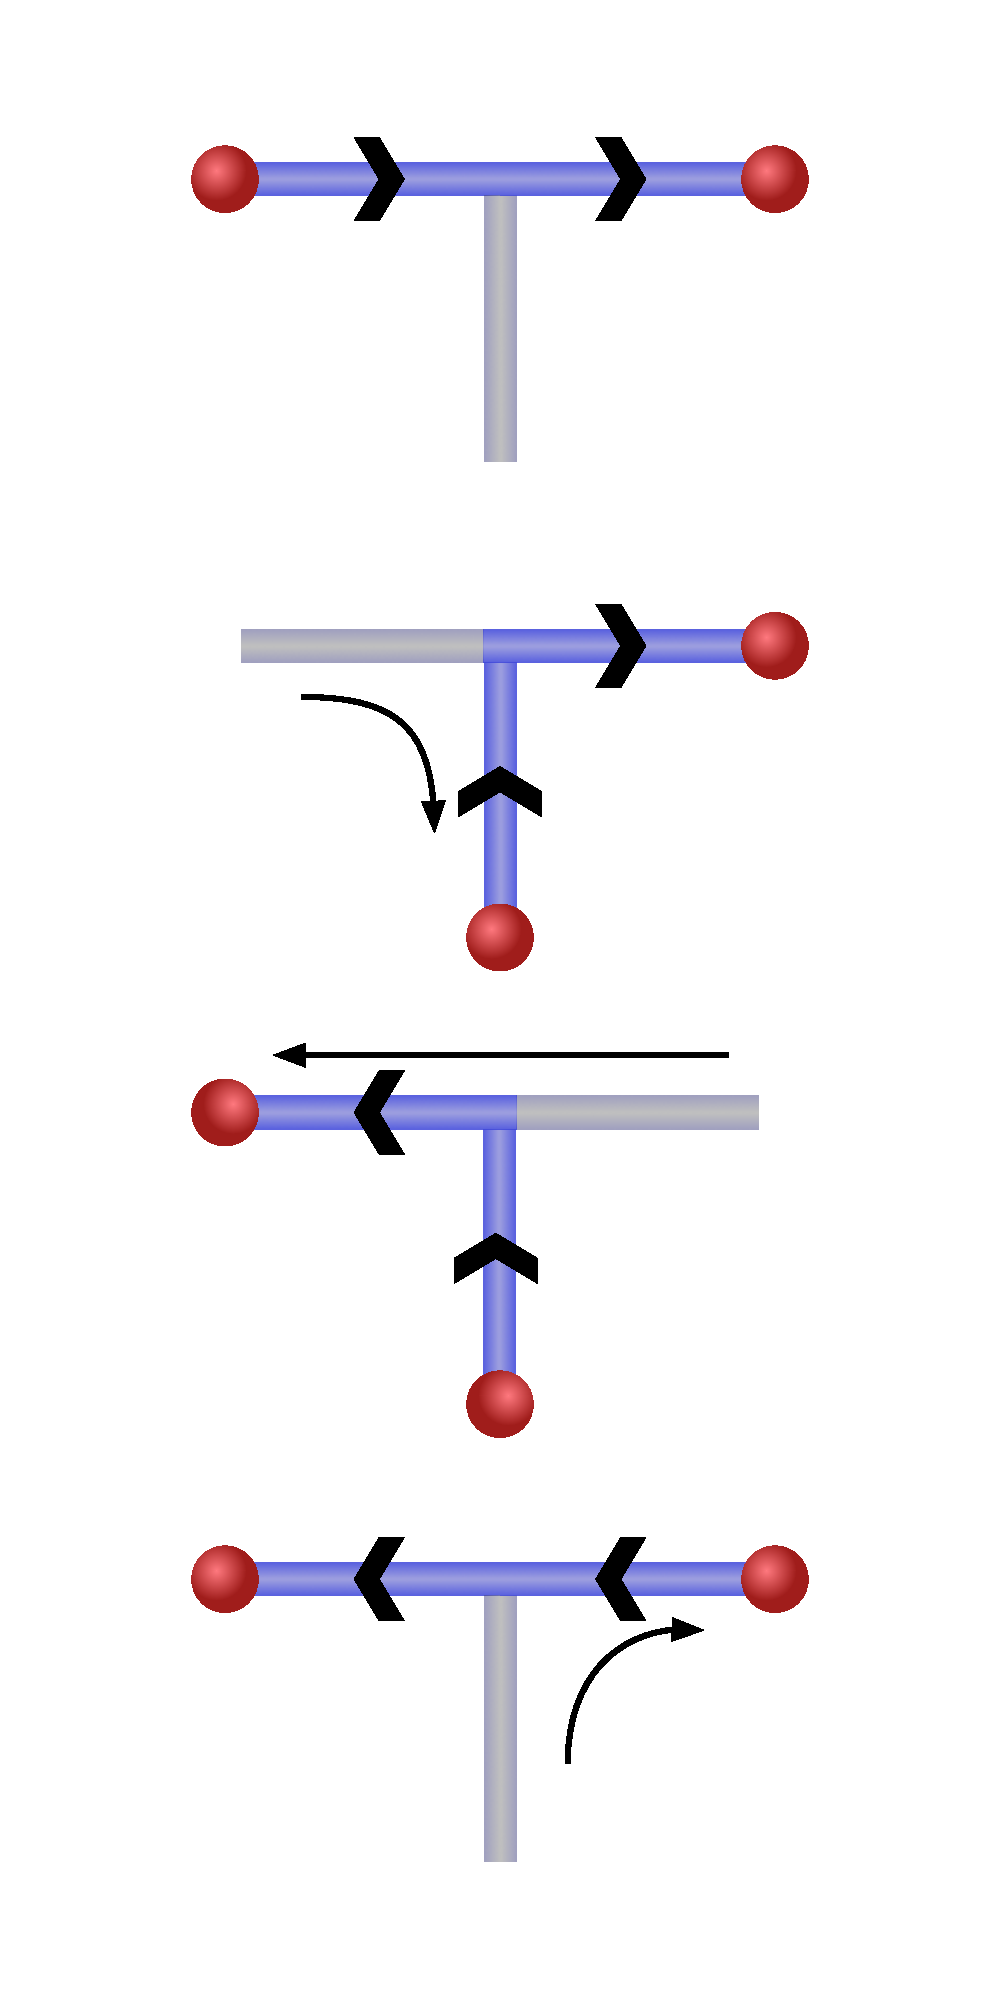
\includegraphics[width=0.4\textwidth]{../../images/t-junction.pdf}
    \end{figure}
    \end{multicols}
  \end{frame}

  \begin{frame}
    \frametitle{\MO}
    \begin{multicols}{2}

    \begin{itemize}
      \item Consider triangular islands which are topologically similar to T-junctions 
      \item Islands of three-fold rotational symmetry occur naturally in epitaxial growth on close-packed metal surfaces
    \end{itemize}

    \begin{figure}
      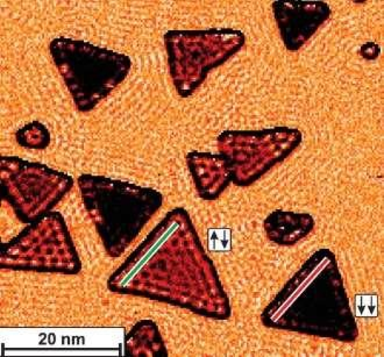
\includegraphics[width=0.5\textwidth]{../../images/triangular-islands.pdf}
    \end{figure}
    \end{multicols}
  \end{frame}

  \section{\DE}
  \begin{frame}
    \frametitle{\DE}
    Lorem ipsum dolor sit amet, consectetur adipisicing elit, sed do eiusmod tempor incididunt ut labore et dolore magna aliqua.
  \end{frame}

  \begin{frame}
    \frametitle{\DE}
    Lorem ipsum dolor sit amet, consectetur adipisicing elit, sed do eiusmod tempor incididunt ut labore et dolore magna aliqua.
  \end{frame}

  \begin{frame}
    \frametitle{\DE}
    Lorem ipsum dolor sit amet, consectetur adipisicing elit, sed do eiusmod tempor incididunt ut labore et dolore magna aliqua.
  \end{frame}

  \begin{frame}
    \frametitle{\DE}
    Lorem ipsum dolor sit amet, consectetur adipisicing elit, sed do eiusmod tempor incididunt ut labore et dolore magna aliqua.
  \end{frame}

  \section{\RE}
  \begin{frame}
    \frametitle{\RE}

    \begin{figure}
      \begin{tikzpicture}
        \draw[help lines,gray!20] (-4,-4) grid[step=0.5] (4,4);

        \node[inner sep=0pt] (figure) at (-1,0)
        {\includegraphics[width=0.5\textwidth]{../../images/wavefunction-1.pdf}};
        \node[inner sep=0pt] (figure) at (3,0) {a figure}
      \end{tikzpicture}
    \end{figure}

  \end{frame}

  \begin{frame}
    \frametitle{\RE}
    Lorem ipsum dolor sit amet, consectetur adipisicing elit, sed do eiusmod tempor incididunt ut labore et dolore magna aliqua.
  \end{frame}

  \section{\CO}
  \begin{frame}
    \frametitle{\CO}
    Lorem ipsum dolor sit amet, consectetur adipisicing elit, sed do eiusmod tempor incididunt ut labore et dolore magna aliqua.
  \end{frame}


%  \begin{frame}
%  \frametitle{List}
%  \begin{itemize}
%  \item Point A
%  \item Point B
%  \begin{itemize}
%  \item part 1
%  \item part 2
%  \end{itemize}
%  \item Point C
%  \item Point D
%  \end{itemize}
%  \end{frame}
%
%  \begin{frame}
%    \frametitle{Enumerate}
%    \begin{enumerate}[]
%  \item Point A
%  \item Point B
%  \begin{enumerate}[i]
%  \item part 1
%  \item part 2
%  \end{enumerate}
%  \item Point C
%  \item Point D
%  \end{enumerate}
%  \end{frame}
%
%  \begin{frame}
%  \frametitle{Using Columns}
%    \begin{columns}
%      \column{0.5\textwidth}
%      Lorem ipsum dolor sit amet, consectetur adipisicing elit, sed do eiusmod tempor incididunt ut labore et dolore magna aliqua.
%      \column{0.5\textwidth}
%      Lorem ipsum dolor sit amet, consectetur adipisicing elit, sed do eiusmod tempor incididunt ut labore et dolore magna aliqua.
%    \end{columns}
%  \end{frame}

\end{document}


